\documentclass[12pt,letterpaper]{article}
\usepackage{graphicx,textcomp}
\usepackage{natbib}
\usepackage{setspace}
\usepackage{fullpage}
\usepackage{color}
\usepackage[reqno]{amsmath}
\usepackage{amsthm}
\usepackage{fancyvrb}
\usepackage{amssymb,enumerate}
\usepackage[all]{xy}
\usepackage{endnotes}
\usepackage{lscape}
\newtheorem{com}{Comment}
\usepackage{float}
\usepackage{hyperref}
\newtheorem{lem} {Lemma}
\newtheorem{prop}{Proposition}
\newtheorem{thm}{Theorem}
\newtheorem{defn}{Definition}
\newtheorem{cor}{Corollary}
\newtheorem{obs}{Observation}
\usepackage[compact]{titlesec}
\usepackage{dcolumn}
\usepackage{tikz}
\usetikzlibrary{arrows}
\usepackage{multirow}
\usepackage{xcolor}
\newcolumntype{.}{D{.}{.}{-1}}
\newcolumntype{d}[1]{D{.}{.}{#1}}
\definecolor{light-gray}{gray}{0.65}
\usepackage{url}
\usepackage{listings}
\usepackage{color}

\definecolor{codegreen}{rgb}{0,0.6,0}
\definecolor{codegray}{rgb}{0.5,0.5,0.5}
\definecolor{codepurple}{rgb}{0.58,0,0.82}
\definecolor{backcolour}{rgb}{0.95,0.95,0.92}

\lstdefinestyle{mystyle}{
	backgroundcolor=\color{backcolour},   
	commentstyle=\color{codegreen},
	keywordstyle=\color{magenta},
	numberstyle=\tiny\color{codegray},
	stringstyle=\color{codepurple},
	basicstyle=\footnotesize,
	breakatwhitespace=false,         
	breaklines=true,                 
	captionpos=b,                    
	keepspaces=true,                 
	numbers=left,                    
	numbersep=5pt,                  
	showspaces=false,                
	showstringspaces=false,
	showtabs=false,                  
	tabsize=2
}
\lstset{style=mystyle}
\newcommand{\Sref}[1]{Section~\ref{#1}}
\newtheorem{hyp}{Hypothesis}

\title{Problem Set 2}
\date{Due: October 22, 2026}
\author{Applied Stats/Quant Methods 1}

\begin{document}
	\maketitle
	\section*{Instructions}
\begin{itemize}
	\item Please show your work! You may lose points by simply writing in the answer. If the problem requires you to execute commands in \texttt{R}, please include the code you used to get your answers. Please also include the \texttt{.R} file that contains your code. If you are not sure if work needs to be shown for a particular problem, please ask.
	\item Your homework should be submitted electronically on GitHub.
	\item This problem set is due before 23:59 on Thursday October 22, 2026. No late assignments will be accepted.

\end{itemize}

	
	\vspace{.5cm}
	\section*{Question 1: Political Science}
		\vspace{.25cm}
	The following table was created using the data from a study run in a major Latin American city.\footnote{Fried, Lagunes, and Venkataramani (2010). ``Corruption and Inequality at the Crossroad: A Multimethod Study of Bribery and Discrimination in Latin America. \textit{Latin American Research Review}. 45 (1): 76-97.} As part of the experimental treatment in the study, one employee of the research team was chosen to make illegal left turns across traffic to draw the attention of the police officers on shift. Two employee drivers were upper class, two were lower class drivers, and the identity of the driver was randomly assigned per encounter. The researchers were interested in whether officers were more or less likely to solicit a bribe from drivers depending on their class (officers use phrases like, ``We can solve this the easy way'' to draw a bribe). The table below shows the resulting data.

\newpage
\begin{table}[h!]
	\centering
	\begin{tabular}{l | c c c }
		& Not Stopped & Bribe requested & Stopped/given warning \\
		\\[-1.8ex] 
		\hline \\[-1.8ex]
		Upper class & 14 & 6 & 7 \\
		Lower class & 7 & 7 & 1 \\
		\hline
	\end{tabular}
\end{table}

\begin{enumerate}
\textbf{(a) Calculate the $\chi^2$ test statistic by hand/manually (even better if you can do "by hand" in \texttt{R}).}\\
\vspace{0cm}
	
	To calculate the chi-square test statistic, I used the formula  $\chi^2 = \sum \frac{(O - E)^2}{E}$. First, I calculated the row and the column totals for the observed frequencies, and put them in a table, shown below.
	
	\lstinputlisting[language=R, firstline=14, lastline=25]{PS02_Solutions_AV.R}  
	
	\begin{table}[!htbp] \centering 
		\caption{Contingency table with marginal totals} 
		\label{tab:polisci_sums} 
		\begin{tabular}{@{\extracolsep{5pt}} ccccc} 
			\\[-1.8ex]\hline 
			\hline \\[-1.8ex] 
			& Not stopped & Bribe requested & Stopped/given warning & Sum \\ 
			\hline \\[-1.8ex] 
			Upper class & $14$ & $6$ & $7$ & $27$ \\ 
			Lower class & $7$ & $7$ & $1$ & $15$ \\ 
			Sum & $21$ & $13$ & $8$ & $42$ \\ 
			\hline \\[-1.8ex] 
		\end{tabular} 
	\end{table} 
	
	Next, I was able to calculate the expected frequencies using the formula:
	\[ f_e = \frac{\text{Row Total} \times \text{Column Total}}{N} \]
	Where $N$ represents the grand total sample size.
	
	\lstinputlisting[language=R, firstline=34, lastline=40]{PS02_Solutions_AV.R}  
	
	After calculating the expected frequencies, I was able to use the chi-square test statistic formula stated above.
	
	\lstinputlisting[language=R, firstline=42, lastline=44]{PS02_Solutions_AV.R}  
	
	I calculated a chi-square statistic of 3.79 (3 s.f.).
	
\textbf{(b) Now calculate the p-value from the test statistic you just created (in \texttt{R}).\footnote{Remember frequency should be $>$ 5 for all cells, but let's calculate the p-value here anyway.}  What do you conclude if $\alpha = 0.1$?}\\
	
	To calculate the p-value, I used the built-in R function \texttt{pchisq()}. I used the following formula to calculate the degrees of freedom (df):
	\[ df = (r - 1) \times (c - 1) \]
	Where $r$ represents the number of rows, and $c$ represents the number of columns in the contingency table.
	
	\lstinputlisting[language=R, firstline=50, lastline=59]{PS02_Solutions_AV.R}  
	
	In a chi-square test, null hypothesis states that the variables are independent, whilst the alternative hypothesis states that the variables are dependent. I calculated a p-value of 0.150 (3 s.f.). When $\alpha = 0.1$, we reject the null hypothesis because the p-value is greater than the $\alpha$ value: $0.15 > 0.1$. This means that the variables are not independent.
	
	\newpage
	\textbf{(c) Calculate the standardized residuals for each cell and put them in the table below.}
	\vspace{0cm}
	
	To calculate the standardised residuals, I used the formula:
	\[ z = \frac{f_o - f_e}{\sqrt{f_e (1 - \text{row proportion})(1 - \text{column proportion})}} \]
	
	First, I calculated the row and column proportions, by dividing the sum of each row and column by N (the grand total).
	
	\lstinputlisting[language=R, firstline=70, lastline=72]{PS02_Solutions_AV.R} 
	
	I then adjusted the results, formatting them into a 2x3 grid because the number of rows is different to the number of columns, meaning R cannot multiply them cell-by-cell like usual.
	
	\lstinputlisting[language=R, firstline=74, lastline=75]{PS02_Solutions_AV.R} 
	
	Finally, I was able to put the standardised residuals (rounded to 3 d.p.) into a table (shown below).
	
	\lstinputlisting[language=R, firstline=80, lastline=84]{PS02_Solutions_AV.R} 
	
	\begin{table}[!htbp] \centering 
		\caption{Table of standardised residuals} 
		\label{tab:residuals} 
		\begin{tabular}{@{\extracolsep{5pt}} cccc} 
			\\[-1.8ex]\hline 
			\hline \\[-1.8ex] 
			& Not stopped & Bribe requested & Stopped/given warning \\ 
			\hline \\[-1.8ex] 
			Upper class & $0.322$ & $$-$1.642$ & $1.523$ \\ 
			Lower class & $$-$0.322$ & $1.642$ & $$-$1.523$ \\ 
			\hline \\[-1.8ex] 
		\end{tabular} 
	\end{table} 
	
	
	\vspace{0cm}
	\textbf{(d) How might the standardized residuals help you interpret the results?}  
	
	Standardised residuals show how much the data in each cell vary from the model. The lower class has positive residual 1.642, meaning they experienced more bribe requests than expected. Conversely, the upper class has a negative residual -1.642, meaning they experienced fewer bribe requests than expected. Upper class was stopped but let off with a warning more often than expected, while the lower class was was stopped and let go less often than expected. Both residuals for upper and lower class in the stopped category are very close to zero, showing they approximately match the expected frequencies in this category. Critical threshold $= +/- $ 1.96. None of the adjusted residuals breach the threshold, meaning that, while there are apparent trends in stopping/bribe requests/warnings across upper and lower classes, these deviations are not statistically significant. These trends observed could be due to random chance.
	
\end{enumerate}
\newpage

\section*{Question 2: Economics}
Chattopadhyay and Duflo were interested in whether women promote different policies than men.\footnote{Chattopadhyay and Duflo. (2004). ``Women as Policy Makers: Evidence from a Randomized Policy Experiment in India. \textit{Econometrica}. 72 (5), 1409-1443.} Answering this question with observational data is pretty difficult due to potential confounding problems (e.g. the districts that choose female politicians are likely to systematically differ in other aspects too). Hence, they exploit a randomized policy experiment in India, where since the mid-1990s, $\frac{1}{3}$ of village council heads have been randomly reserved for women. A subset of the data from West Bengal can be found at the following link: \url{https://raw.githubusercontent.com/kosukeimai/qss/master/PREDICTION/women.csv}\\

\noindent Each observation in the data set represents a village and there are two villages associated with one GP (i.e. a level of government is called "GP"). Figure~\ref{fig:women_desc} below shows the names and descriptions of the variables in the dataset. The authors hypothesize that female politicians are more likely to support policies female voters want. Researchers found that more women complain about the quality of drinking water than men. You need to estimate the effect of the reservation policy on the number of new or repaired drinking water facilities in the villages.
\vspace{.5cm}
\begin{figure}[h!]
	\caption{\footnotesize{Names and description of variables from Chattopadhyay and Duflo (2004).}}
	\vspace{.5cm}
	\centering
	\label{fig:women_desc}
	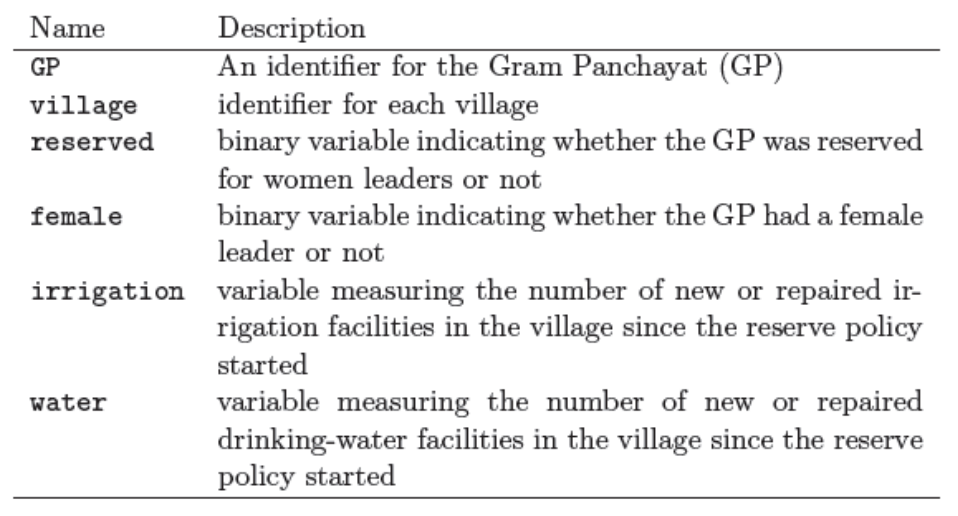
\includegraphics[width=1.1\textwidth]{women_desc.png}
	
\end{figure}		

\newpage
\begin{enumerate}
	\item [(a)] State a null and alternative (two-tailed) hypothesis. 
	
	Null hypothesis: the reservation policy had no effect on the number of new or repaired drinking water facilities in the villages, $\mu = 0$
	
	Alternative hypothesis: the reservation policy did have an effect on the number of new or repaired drinking water facilities in the villages, $\mu \neq 0$
	
	\vspace{0cm}
	\item [(b)] Run a bivariate regression to test this hypothesis in \texttt{R} (include your code!).
	
	I used the built-in R function \texttt{lm()} to run a bivariate regression to test the above null hypothesis.
	
	\lstinputlisting[language=R, firstline=126, lastline=135]{PS02_Solutions_AV.R} 
	
	The p-value is less than standard significance threshold: $0.0197 < 0.05$. As such, we reject the null hypothesis in favour of the alternative hypothesis, meaning that there is enough statistical evidence to suggest that the reservation policy had an effect on the drinking water facilities in these villages.
	
	\vspace{0cm}
	\item [(c)] Interpret the coefficient estimate for reservation policy. 
	
	The coefficient estimate is: $\beta$ = 9.252. This shows that the reservation policy had a positive effect, meaning that there were more drinking water facilities due to the reservation policy. In other words, villages that were randomly selected to have have their GP reserved for female leaders built or repaired 9.252 more drinking water facilities than villages without the reservation policy.
	
\end{enumerate}


%\end{enumerate}
\end{document}
